

\section{Introduction}


%State your problem and provide the motivation for solving/studying it: Why is
%the problem important? In which field of computer science does it fit?  What
%novel contribution does your project make? Your introduction should end with a
%brief outline for the organization of the rest of the paper. This section
%should be approximately 1 page in length.

In the the last ten years the popularization of 3D printers and makerspaces has caused interest in digital fabricators to blossom. Digital fabricators are machines which use computer controlled tools to produce 3D objects. The digital fabrication workflow entails a computer-aided design (CAD) process where the user produces electronic schematics. These schematics are then brought into a computer-aided manufacturing (CAM) program where the user creates tool paths for the machine, the output of this process is instructions for the fabrication machine. Finally these instructions are uploaded to the digital fabricator and the schematic is fabricated in the medium worked by the fabrication machine. 

\begin{figure}[h]
  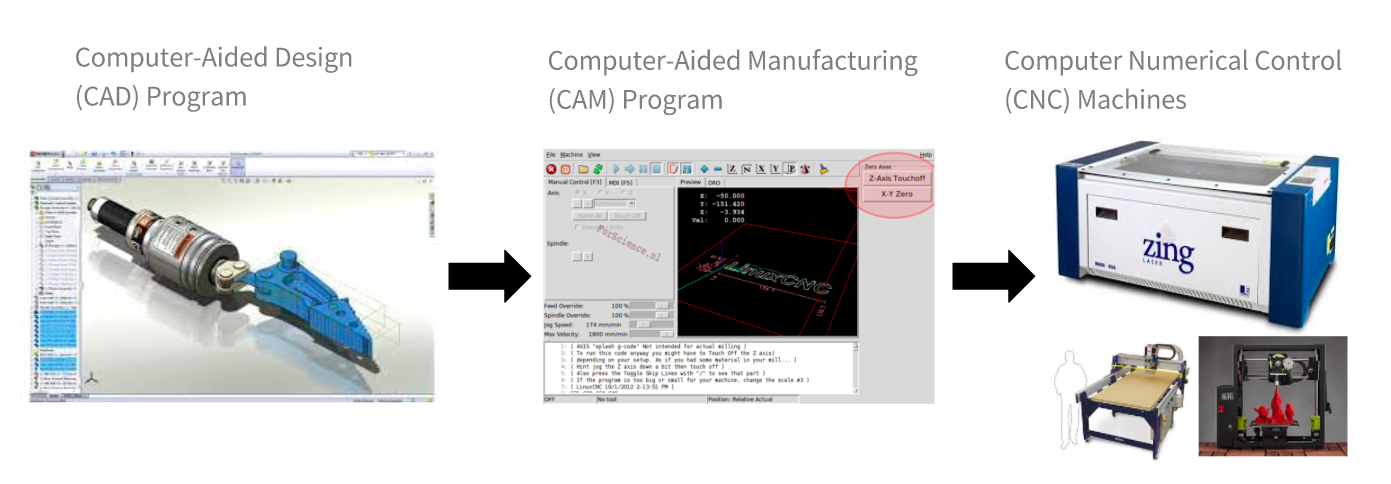
\includegraphics[width=\linewidth]{digiFabWorkflow.jpg}
  \caption{The digital fabrication workflow.}
  \label{fig:digiFabWorkflow}
\end{figure}

Personal digital fabricators, or fabricators intended for use by a large audience (in contrast to industrial digital fabricators), include 3D printers, computer-numerical-control (CNC) mills, and laser cutters. Laser cutters are often considered the best balance of accessibility and usefulness of these digital fabricators. A laser cutter works by focusing a high powered laser through a focusing head which is attached to a gantry. The gantry controls the position of the head and therefore the location of the laser on a workpiece that rests on a bed underneath the gantry.

\begin{figure}[h]
  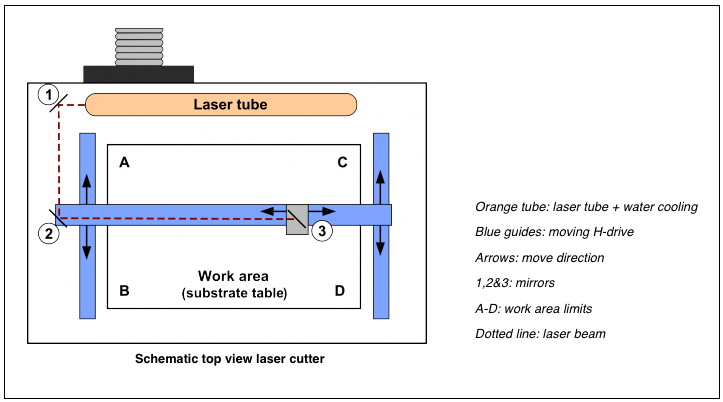
\includegraphics[width=\linewidth]{lasersystem.jpg}
  \caption{Top view schematic of laser cutter.}
  \label{fig:lasersystem}
\end{figure}

Laser cutters are capable of cutting and engraving. Most commercial laser cutters will cut plastic, paper, cardboard, and wood up to a quarter inch. They can also engrave all these materials and most types of metal and glass.

There are two main paradigms for modeling in CAD programs - direct modeling and parametric modeling. In direct modeling the user interacts directly with the geometry. This is typically through transformations such as dragging, rotating, or scaling. In parametric modeling the design program utilizes a geometric constraint solver that allows the user to specify constraints and dimensions on geometry. The design is then automatically adjusted to satisfy these constraints when the user modifies geometry directly. Figure X depicts the common constraint capabilities of a parametric design program.

\begin{figure}[h]
  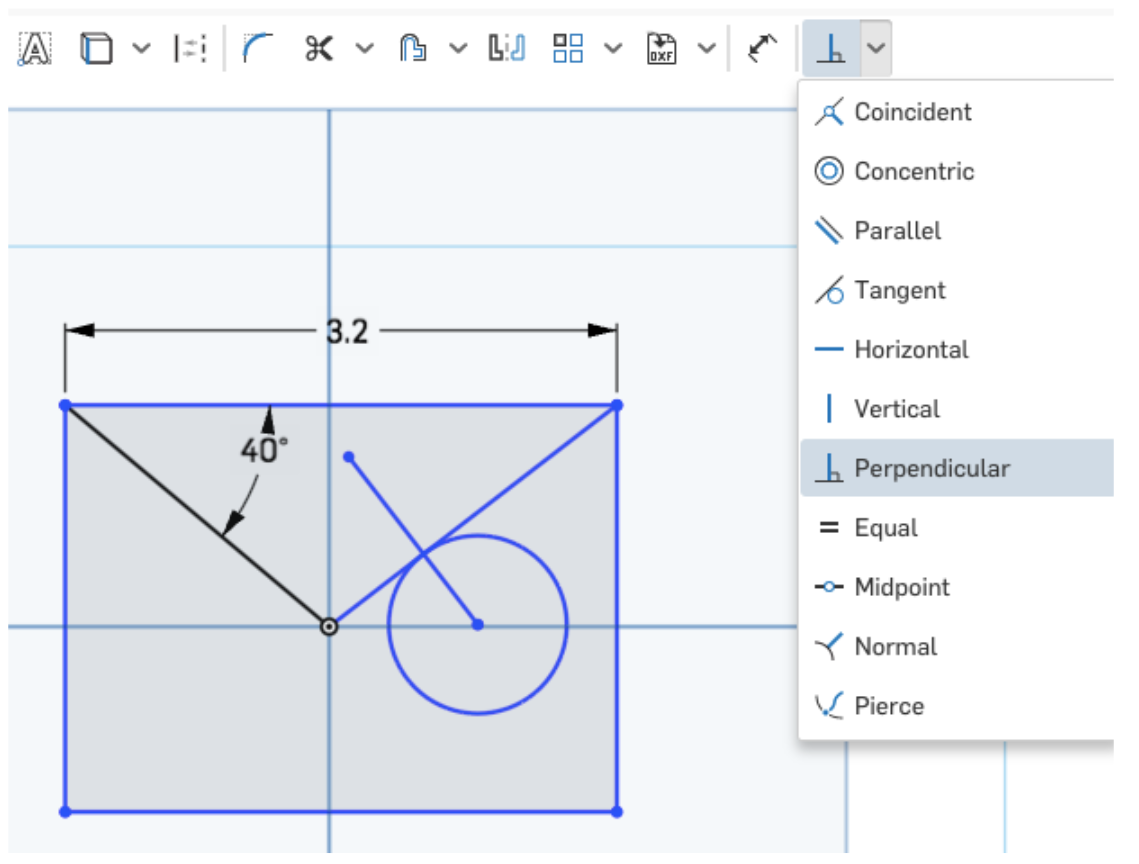
\includegraphics[width=\linewidth]{parametricProgram.jpg}
  \caption{Screenshot of parametric CAD program (Onshape) which shows common geometric constraints.}
  \label{fig:parametricProgram}
\end{figure}

Laser cutters are typically 2-dimensional fabricators which means there is no $z$-axis adjustability during fabrication. Consequently, prevalent drawing programs such as Adobe Illustrator and CorelDRAW were adopted for creating designs intended for laser cutting. Vector graphics, a scale-agnostic format where images are represented mathematically, are typically used for generating cutting paths. Rasters, a format where images are represented by pixels, are typically interpreted as engravings when laser cutting.